\documentclass[12]{article}
%\usepackage[utf8]{inputenc}
\usepackage{mathtools, amssymb, extarrows, bm, dsfont, amsmath}
\usepackage{tikz}
\usepackage{tikzit}
\input{tikz.tikzstyles}
\usepackage{pgfplots}
\usepackage{setspace}
\usepackage{algorithm}
\usepackage{algpseudocode}
\usepackage[shortlabels]{enumitem}
\usepackage{hyperref}
\hypersetup{
	colorlinks=true,
	linkcolor=blue,
	filecolor=magenta,      
	urlcolor=cyan,
	pdftitle={Overleaf Example},
	pdfpagemode=FullScreen,
}
\usepackage{geometry}
\geometry{
	a4paper,
	total={140mm,257mm},
	left=35mm,
	top=20mm,
}
\usepackage{subcaption}
\usepackage{graphicx}
\usepackage{float}
\usepackage{multirow}
\usepackage{changepage}
\usepackage{import}

\newcommand{\myskip}{0.7em}
\newcommand{\prob}{{\mathbb P}}
\newcommand{\E}{{\mathbb E}}
\newcommand{\Var}{\mathrm{Var}}
\newcommand{\Cov}{\mathrm{Cov}}
\newcommand{\Corr}{\mathrm{Corr}}
\DeclareMathOperator*{\argmax}{arg\,max}
\DeclareMathOperator*{\argmin}{arg\,min}
%\renewcommand\thesection{Q\arabic{section}}
\pgfplotsset{
	standard/.style={%Axis format configuration
		axis x line=middle,
		axis y line=middle,
		enlarge x limits=0.15,
		enlarge y limits=0.15,
		every axis x label/.style={at={(current axis.right of origin)},anchor=north west},
		every axis y label/.style={at={(current axis.above origin)},anchor=north east},
		every axis plot post/.style={mark options={fill=white}}
	}
}

%%%%%%%%%%%%%%%%%%%%%%%%%%%%%%%%%%%%%%%%%%%%%%%%%%%%%%%%%%%%%%%%%%%%%%%%%%%%
\title{
	\rule{\linewidth}{2.5pt}\\
	\textbf{{\LARGE Security and Privacy in Machine Learning}}\\
	{\Large Homework 3}\\[-.35em]
	\rule{\linewidth}{0.75pt}%\\
%	{\normalsize Spring 2023}
}
\author{{Javad Hezareh}\\{98101074}\\[1em]Spring 2023}
\date{}

\onehalfspacing
\begin{document}
	\maketitle
	\vspace{15mm}
	\tableofcontents
	
	\pagebreak
	\section{Adversarial Training of Linear Classifiers}
	\begin{enumerate}[label=\textbf{(\alph*)}]
		\item
		Yes, even in this simple linear classifier it is possible to have adversarial examples. If we add a small perturbation like $\bm{\delta}$ to the input, then the model output will be:
		\[
		\bm{\tilde{x}} = \bm{x} + \bm{\delta} \implies h(\bm{\tilde{x}}) = \bm{W}^T(\bm{x} + \bm{\delta}) + b \implies h(\bm{\tilde{x}}) - h(\bm{x}) = \bm{W}^T\bm{\delta}
		\]
		Therefore the output change depends on $\bm{\delta}$ and $\bm{W}$. Let $\bm{\delta} = \epsilon\;\text{sign}(\bm{W})$, then we know $\|\bm{\delta}\|_{\infty} \le \epsilon$ and we have:
		\[
		h(\bm{\tilde{x}}) - h(\bm{x}) = \epsilon\bm{W}^T \text{sign}(\bm{W}) = \epsilon\|\bm{W}\|_1
		\]
		As we do not have any bound on the value of $\|\bm{W}\|_1$, then we can have significant change in the output by small perturbation of input if this value be very large.
		\item
		We know the original form of optimization in adversarial training is
		\[
		\min_{\bm{W}, b} \E\left[\max_{\bm{\delta} \in \Delta} \mathcal{L}\left(h(\bm{x}+\bm{\delta}), y\right)\right]
		\]
		where $\Delta = \left\{\bm{\delta}\in \mathbb{R}^n  \middle| \|\bm{\delta}\|_\infty \le \epsilon\right\}$. Now if want to solve the inner maximization problem using FGSM attack, then we have:
		\[
		\begin{aligned}
			\bm{\delta}_{\text{FGSM}} &= \epsilon\;\text{sign}\left(\nabla_{\bm{x}} \mathcal{L}\left(h(\bm{x}), y\right)\right) \\[\myskip]
				&= \epsilon\;\text{sign}\left(\nabla_{\bm{x}} \log\left(1+e^{-yh(\bm{x})}\right)\right) \\[\myskip]
				&= \epsilon\;\text{sign}\left(\frac{-y e^{-yh(\bm{x})}}{1+e^{-yh(\bm{x})}}\nabla_{\bm{x}} h(\bm{x})\right) \\[\myskip]
				&= \epsilon\;\text{sign}\left(\frac{-y e^{-yh(\bm{x})}}{1+e^{-yh(\bm{x})}} \bm{W}\right) \\[\myskip]
				&= \epsilon\;\text{sign}\left(\alpha\bm{W}\right)\qquad\quad \alpha = \frac{-y e^{-yh(\bm{x})}}{1+e^{-yh(\bm{x})}}
		\end{aligned}
		\]
		Applying this value in the loss function we have:
		\[
		\begin{aligned}
			\mathcal{L}(h(\bm{x}+\bm{\delta}_\text{FGSM}), y) &\approx \mathcal{L}(h(\bm{x}), y) + (\delta_\text{FGSM})^T\nabla_{\bm{x}}\mathcal{L} \\[\myskip]
				&\approx \mathcal{L}(h(\bm{x}), y) + \epsilon\; \alpha\bm{W}^T\text{sign}(\alpha\bm{W}) =\mathcal{L}(h(\bm{x}), y) + \epsilon\|\alpha\bm{W}\|_1
		\end{aligned}
		\]
		Therefore the adversarial training objective for this problem will be:
		\[
		\min_{\bm{W}, b} \E\left[\mathcal{L}(h(\bm{x}), y) + \epsilon\|\alpha\bm{W}\|_1\right]
		\]
		\item
		If we use $l_1$ regularizer, then the training objective will be:
		\[
		\min_{\bm{W}, b} \E\left[\mathcal{L}(h(\bm{x}), y) + \gamma\|\bm{W}\|_1\right]
		\]
		As we can see this objective is very similar to the one we have in adversarial training except that $\alpha$ multiplier. As we saw in part (a), the reason we have adversarial examples is the $l_1$-norm of weight matrix hence using $l_1$ regulizer or a version of that such as what we have in the objective of adversarial training will lead to a model which is robust to adversarial examples.
	\end{enumerate}

	\pagebreak
	\section{Targeted Attack}
	\begin{enumerate}[label=\textbf{(\alph*)}]
		\item We can perform targeted attack for different classes and then choose our target class to be the class for which we have the smallest size of perturbation or the largest size. Former method leads to the best case scenario and the later one leads to the worst case scenario. 
		\item
		Let's say our target class is $t$, then we want to build an adversarial input on which our model performs well. Therefore we want to minimize the loss function on this target class:
		\[
		x_{adv} = \argmin_{x^\prime} \mathcal{L}(h_w(x^\prime), t)
		\]
	\end{enumerate}

	\pagebreak
	\section{Various Attacks}
	To build adversarial examples using PGD we need to perform following steps:
	\begin{algorithm}[H]
		\caption{PGD attack}
		\begin{algorithmic}
			\State $x:=$ input, $k :=$ number of steps, $\alpha :=$ step size, $\epsilon :=$ attack radius \\
			\State $x^0 = U(x-\epsilon, x+\epsilon)$
			\For{$t=1 \to k$}
			\State $\delta = \alpha\;\text{sign}\left(\nabla_x \mathcal{L}(h(x^t), y)\right)$
			\State $x^{t} = Proj_{[x-\epsilon, x+\epsilon]}(x^{t-1}+\delta)$
			\State $x^{t} = Clip_{[0, 1]}(x^{t})$
			\EndFor
		\end{algorithmic}
	\end{algorithm}
	\noindent
	Using this method, we will explore $\epsilon$ neighborhood of input step by step instead of just single step like FGSM. However, our steps are still in the direction of the square corners but with smaller step size which enable us to take multiple steps and find a better solution. A sample of performing this algorithm will be as follows:
	\begin{figure}[H]
		\centering
		\tikzfig{pgd}
		\caption{A sample trajectory of performing PGD with $k=4$.}
	\end{figure}
	\noindent
	In FGSM-RS method, everything is just like FGSM but before performing an FGSM attack, first we need to pick a random point in $\epsilon$ neighborhood of input. Its algorithm is as follows:
	\begin{algorithm}[H]
		\caption{FGSM-RS attack}
		\begin{algorithmic}
			\State $x:=$ input, $\alpha:=$ step size, $\epsilon :=$ attack radius
			\\
			\State $x^0 = U(x-\epsilon, x+\epsilon)$
			\State $\delta = \alpha\;\text{sign}\left(\nabla_x \mathcal{L}(h(x_0), y)\right)$
			\State $x_{adv} = Proj_{[x-\epsilon, x+\epsilon]}(x^0 + \delta)$
			\State $x_{adv} = Clip_{[0, 1]}(x_{adv})$
		\end{algorithmic}
	\end{algorithm}
	\noindent
%	A sample of running above algorithm will be as follows:
	\begin{figure}[H]
		\centering
		\tikzfig{fgsm-rs}
		\caption{A sample trajectory of performing FGSM-RS.}
	\end{figure}

	\pagebreak
	\section{Practical}
	In following sections you can find the report of this question:
	\begin{enumerate}
		\item[8:] This part was the evaluation of standard model on adversarial examples using FGSM attack and different $\epsilon$ values.
		\begin{table}[H]
			\centering
%			\caption{Standard trained model accuracy against adversarial attack using FGSM method with different $\epsilon$ values.}
			\begin{tabular}{|c|c|c|}
				\hline
				&\multicolumn{2}{|c|}{Standard ResNet} \\
				\hline\hline
				\multirow{4}{*}{FGSM} & $\epsilon$ & Adversarial Accuracy \\
				\cline{2-3}
				& $4/255$ & 10 \% \\
				\cline{2-3}
				& $8/255$ & 1.6 \% \\
				\cline{2-3}
				& $12/255$ & 0.6 \% \\
				\hline
			\end{tabular}
		\end{table}
		We can see that as we expect the standard model is not robust against FGSM adversarial attack.
		\item[9:]
		Following is the 5 crafted adversarial examples using FGSM and $\epsilon = 8/255$:
		\begin{figure}[H]
			\centering
			\begin{tabular}{|c|c|c|}
				\hline
				True label & Predicted Label & Confidence \\
				\hline
				cat & dog & 0.72 \\
				ship & car & 0.64 \\
				ship & bird & 0.99 \\
				plane & ship & 0.99 \\
				frog & dear & 0.99 \\
				\hline
			\end{tabular}
		\end{figure}
		\item[10:] In figure \ref{fig:fgsm-attack} you can find the crafted adversarial examples and their clean inputs.
		\begin{figure}[H]
			\centering
			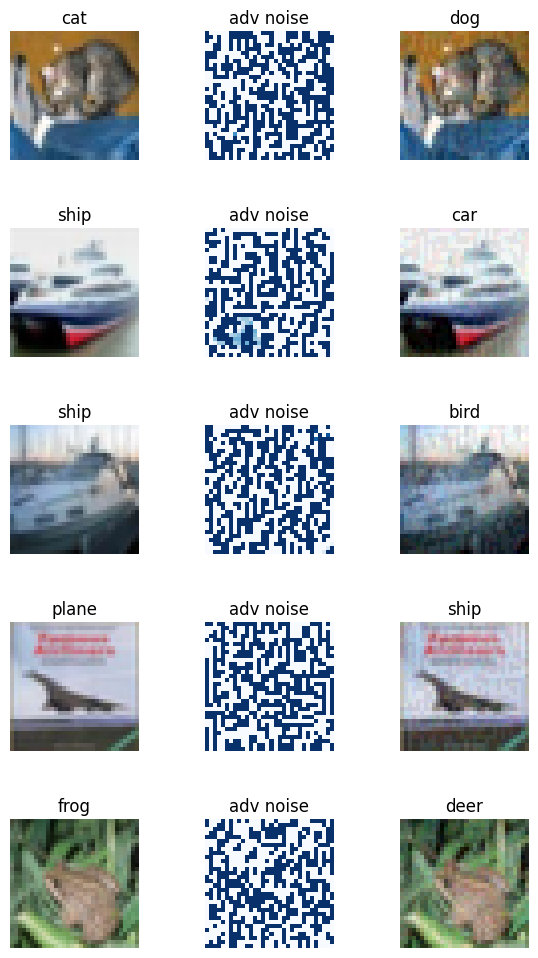
\includegraphics[width=0.45\textwidth]{./figures/practical-fgsm.png}
			\caption{Crafted adversarial examples using FGSM and $\epsilon = 8/255$.}
			\label{fig:fgsm-attack}
		\end{figure}
		\item[11:] In this part we used adversarial training to build a robust model against adversarial perturbations. The results of adversarial trained model are as follows:
		\begin{figure}[H]
			\centering
			\begin{tabular}{|c|c|}
				\hline
				\multicolumn{2}{|c|}{AT ResNet} \\
				\hline\hline
				Test data & Accuracy \\
				\hline
				Clean & 76.01 \% \\
				FGSM & 39.97 \%\\
				\hline
			\end{tabular}
		\end{figure}
		\item[13:] In this part we used PGD attack to evaluate the robustness of standard and adversarial trained model:
		\begin{figure}[H]
			\centering
			\begin{tabular}{|c|c|c||c|c|}
				\hline
				& \multicolumn{2}{|c||}{Standard ResNet} & \multicolumn{2}{|c|}{AT ResNet} \\
				\hline\hline
				\multirow{3}{*}{PGD} & $k$ & Accuracy & $k$ & Accuracy \\
				\cline{2-5}
				& 2 & 5.31 \% & 2 & 62.96 \% \\
				\cline{2-5}
				& 4 & 0.19 \% & 4 & 58.60 \% \\
				\hline
			\end{tabular}
		\end{figure}
		\item[14:] In figure \ref{fig:pgd-attack} you can see the crafted adversarial examples using PGD:
		\begin{figure}[H]
			\centering
			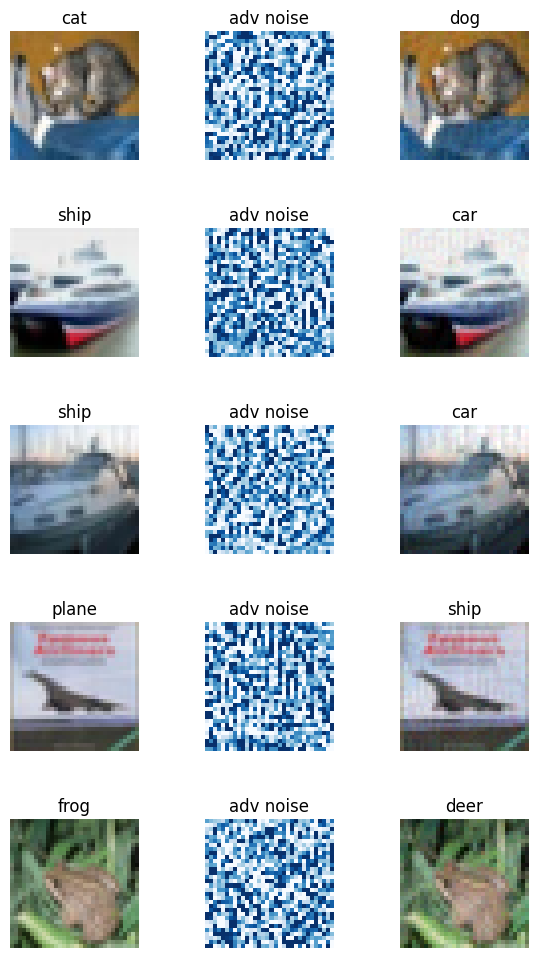
\includegraphics[width=0.45\textwidth]{./figures/practical-pgd.png}
			\caption{Crafted adversarial examples using PGD, $\epsilon = 8/255$ and $k=4$.}
			\label{fig:pgd-attack}
		\end{figure}
		\item[15:] By adding Gaussian noise with mean 0 and variance of $6/255$ to the test data we have:
		\begin{table}[H]
			\centering
			\begin{tabular}{|c|c|c|}
				\hline
				Accuracy & Std ResNet & AT ResNet \\
				\hline
				Noise & 34.21 \% & 73.09 \% \\
				\hline 
			\end{tabular}
		\end{table}
		\noindent
		We can see that adversarial trained model perform better on noisy images. This behavior is expected, cause the decision boundary of adversarial trained model are not very tight to data points and therefore by moving randomly in their neighborhood the decision will not change.
		\item[16:] The resulted diagrams are as follows:
		\begin{figure}[H]
			\centering
			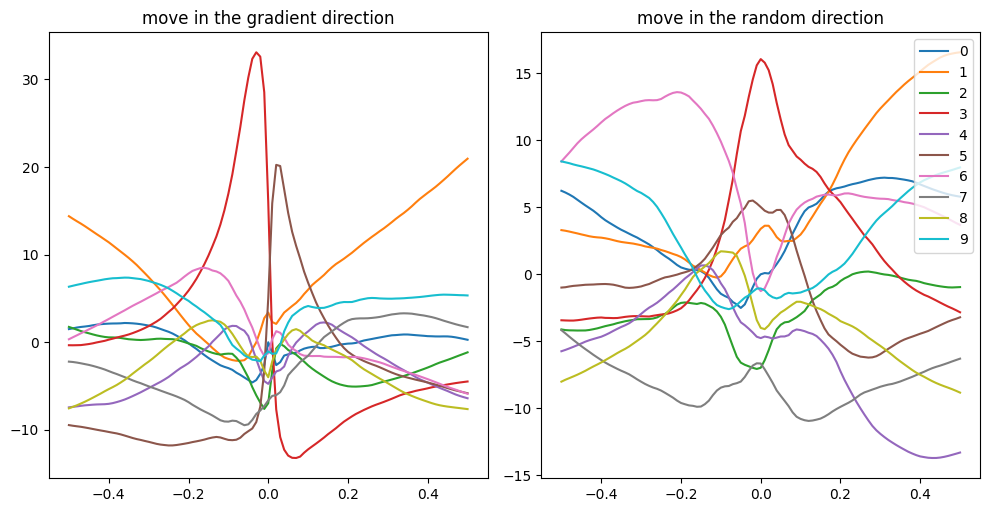
\includegraphics[width=0.9\textwidth]{./figures/logit-epsilon.png}
			\caption{The change in logits by changing $\epsilon$.}
			\label{fig:diagrams}
		\end{figure}
		\noindent
		The image that we have calculated this diagrams on that was the picture of a cat which is the 4-th class, or the class with index 3. As we saw in previous parts by using FGSM attack, this picture was labeled as a dog which is 6-th class or the class with index 5. We can adjust this behavior by graphs in figure \ref{fig:diagrams}, if we move in the direction of gradient, the logit related to class 3 (red line) decrease significantly and the logit related to class 5 (brown line) increase. This leads model to predict dog as output. But when we move in random direction this phenomena can not happen, cause by small changes in $\epsilon$, no significant change in the logits happen and still model predict its previous predictions.
	\end{enumerate}
\end{document}
